\chapter{Membangun Model Prediksi}

\section{Binary Classification}
	Binary Classification biasanya melibatkan satu kelas yang mana dalam keadaan normal dan kelas lainnya yang merupakan keadaan abnormal atau dapat berarti binary classification berupa kelas positif dan kelas negatif. Contohnya, pada email terdeteksi spam email, ada keadaan dimana email tersebut dapat berupa spam atau bukan.  Misalnya bukan spam berarti keadaan normal dan spam berarti keadaan abnormal. Kelas dengan keadaan normal atau positif diberi label kelas 0 dan kelas dengan keadaan abnormal atau negatif diberi label kelas 1. 
	\newline Adapun Algoritma yang digunakan untuk binary classification antaralain sebagai berikut :
	\begin{enumerate}
		\item Decision Trees
		\item Support Vector Machine
		\item Naive Bayes
		\item Logistic Regression
		\item K-Nearest Neighbors
	\end{enumerate}

	\begin{figure}[!htbp]
		\centering
		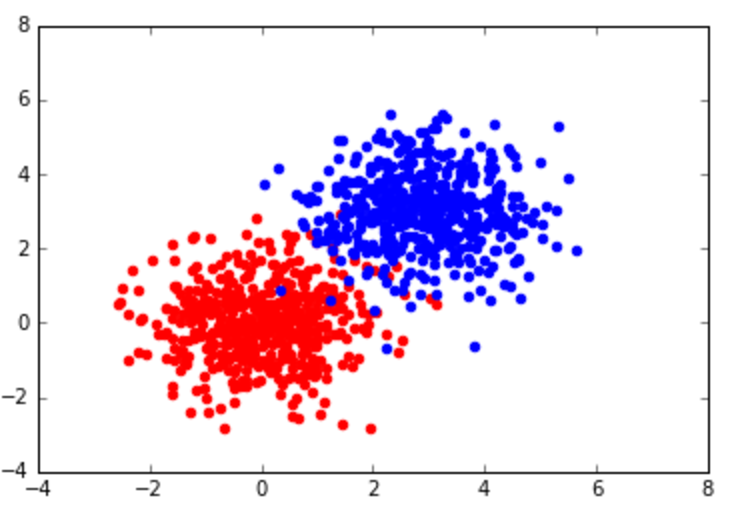
\includegraphics[width=9cm,height=7cm]{figures/Cp2-binaryClassification.png}
		\caption{Binary Classification}
	\end{figure}

	\section{Supervised Learning, Unsupervised Learning dan Clustering }
	\begin{enumerate}
        \item Supervised Learning
        \newline Supervised Learning merupakan sebuah pemodelan dimana algoritmanya dapat membangkitkan suatu fungsi yang memetakan input ke output yang diinginkan. Pada Supervised Learning kita mengolah data yang memiliki label sehingga tujuan pengolahan tersebut adalah mengelompokkan data ke data yang sudah ada. Supervised Learning dalam kehidupan sehari-hari bisa ditemukan pada kasus prediksi harga saham, klasifikasi pelanggan, klasifikasi gambar dan lain-lain.

		\begin{figure}[!htbp]
			\centering
			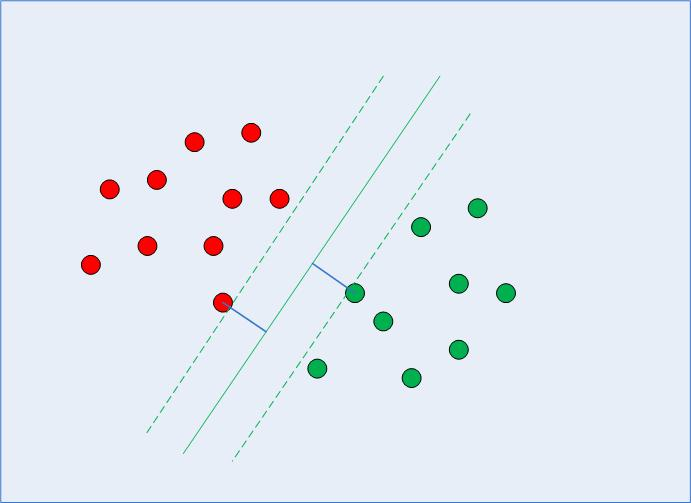
\includegraphics[width=9cm,height=7cm]{figures/Cp2-SVM.png}
			\caption{Supervised Learning : SVM Model Using Linear Kernel}
			\label{penanda}
		\end{figure}

        \item Unsupervised Learning
        \newline Unsupervised Learning merupakan sebuah pemodelan dimana algoritmanya memodelkan sekumpulan input secara otomatis tanpa adanya panduan output yang diinginkan. Unsupervised Learning kita mengolah data yang tidak memiliki label, sehingga tujuan kita dalam menggunakan Unsupervised Learning adalah mengelompokkan suatu data yang hampir sama dengan data tertentu.
		\newline Adapun Algoritma yang digunakan untuk Unsupervised Learning antaralain sebagai berikut :
		\begin{enumerate}
		\item K-means
		\item Hierarchical Clustering
		\item DBSCAN
		\item Fuzzy C-Means
		\item Self-Organizing Map
	\end{enumerate}

        \item Clustering
        \newline Clustering adalah metode pengelompokan objek sedemikian rupa sehingga objek dengan fitur serupa berkumpul, dan objek dengan fitur yang berbeda berpisah. Ini adalah teknik umum untuk analisis data statistik untuk pembelajaran mesin dan penggalian data. Analisis data eksplorasi dan generalisasi juga merupakan area yang menggunakan clustering.
        \end{enumerate}

	\section{Evaluasi dan Akurasi}
	Evaluasi merupakan kegiatan yang dilakukan untuk mengukur seberapa baik sebuah model dapat bekerja dengan menghitung akurasinya. Akurasi merupakan ukuran atau persentase data yang diklasifikasikan dengan benar. Akurasi klasifikasi juga dapat berarti membagi jumlah prediksi benar terhadap total prediksi. Dalam model klasifikasi, dapat diprediksi nilai terbesar dan memberikan akurasi yang tinggi serta model yang dihasilkan dapat memprediksi nilai yang salah. Sehingga dalam hal ini dibutuhkan adanya metrik evaluasi yang dapat mengukur peforma dari model klasifikasi yang sudah dibuat. Metrik yang digunakan adalah Precision, Recall dan Confusion Matrix.

	\section{Confusion Matrix}
	Confusion Matrix adalah pengukuran performa untuk masalah klasifikasi machine learning dimana keluaran dapat berupa dua kelas atau lebih. Confusion Matrix adalah tabel dengan 4 kombinasi berbeda dari nilai prediksi dan nilai aktual.
	\newline 
	\textbf {Berikut adalah contoh dari confusion matrix :}
	\begin{enumerate}
		\item Accuracy
		\item Precision (Positive Predictive Value)
		\item Recall atau Sensitivity (True Positive Rate)
	\end{enumerate}
	\textbf {Cara membuat dan membaca confusion matrix}
	
	\begin{figure}[!htbp]
		\centering
		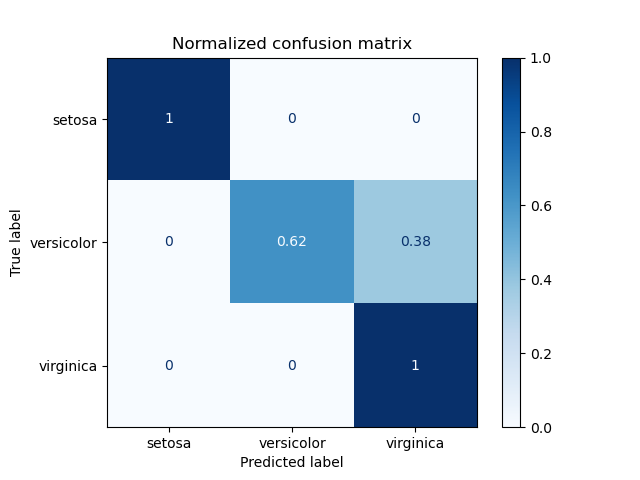
\includegraphics[width=9cm,height=7cm]{figures/Cp2-ConfusionMatrix.png}
		\caption{Confusion Matrix}
		\label{penanda}
	\end{figure}

	\section{K-fold cross validation}
	K-fold cross validation merupakan model evaluasi atau prosedur yang akan memisahkan antara data training dan data testing. K-fold cross validation dapat di definisikan sebagai pengujian cross validation yang digunakan untuk menilai kinerja dari sebuah metode algoritma dengan membagi sampel data secara acak dan mengelompokkan data tersebut sebanyak nilai K k-fold.
	\begin{figure}[!htbp]
		\centering
		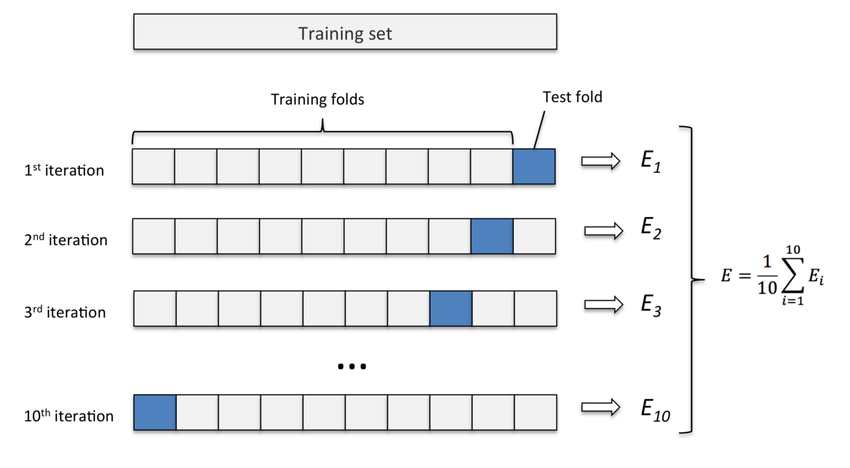
\includegraphics[width=9cm,height=7cm]{figures/Cp2-K-fold cross validation.png}
		\caption{K-fold cross validation}
		\label{penanda}
	\end{figure}
	\newline
	\textbf {Cara kerja K-fold cross validation : }
	\begin{enumerate}
		\item Tentukan instance, dibagi menjadi N bagian atau misalnya ada 10 data dan akan dilakukan K-fold cross validation pada data tersebut.
		\item Data dibagi menjadi data testing untuk pengujian pada model dan data training untuk melatih model. 
		\item Menentukan nilai K, misalnya dalam hal ini ditentukan nilai K = 10 dimana data tersebut nantinya akan ada 10 lipatan atau disebut dengan fold
	\end{enumerate}

	\section{Decision Tree}
	Decision Tree merupakan metode penbelajaran non parametrik yang digunakan untuk klasifikasi dan regresi. Tujuan dari decision tree adalah membuat model yang akan memprediksi nilai variable dengan mempelajari aturan keputusan sederhana yang disimpulkan dari sebuah fitur data. Decision tree merupakan struktur yang sama seperti diagram alur dimana simpul internal sebagai fitur atau atribut, cabang sebagai aturan dan keputusan, serta setiap simpul daun akan mewakili hasilnya.
	\begin{figure}[!htbp]
		\centering
		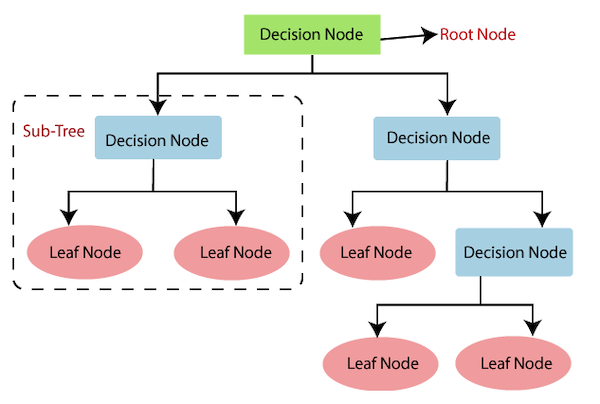
\includegraphics[width=9cm,height=7cm]{figures/Cp2-DecisionTree.png}
		\caption{Decision Tree}
		\label{penanda}
	\end{figure}

	\section{Information Gain dan Entropi}
	\begin{enumerate}
	\item Entropi
	\newline  Entropy merupakan ukuran ketidakpastian. Semakin besar nilai informasi gain dari suatu atribut, maka semakin signifikan atribut tersebut untuk tugas prediksi. Sebuah objek yang di akan di klasifikasikan ke dalam decision tree harus di uji nilai entropinya. Entropi merupakan ukuran dari informasi yang dapat mengetahui karakteristik  dari dari impuryt ,dan homogenity dari sekumpulan data. Entropi juga merupakan jumlah bit yang diperkirakan akan dibutuhkan untuk mengekstrak suatu kelas dari data acak pada suatu ruang sampel. Dari nilai entropi tersebut kemudian akan dihitung information gain masing-masing atribut. 

	\item Information Gain
	\newline Metode Information Gain adalah metode yang menggunakan teknik scoring untuk pembobotan sebuah fitur dengan menggunakan maksimal entropy. Fitur yang dipilih adalah fitur dengan nilai Information Gain yang lebih besar atau sama dengan nilai threshold tertentu. Kemudian setelah mendapatkan nilai entropi untuk suatu kumpulan data, maka akan diukur efektivitas nya atau disebut dengan information gain. Information gain digunakan untuk mengukur seberapa besar relevan atau pengaruh sebuat feature terhadap hasil pengukuran. Information Gain dikenal juga dengan sebutan Mutual Information dalam kasus untuk mengetahui dependency antara dua variable (x,y).
	\end{enumerate}


\section{Praktikum}
	\subsection{Scikit-Learn}
\begin{enumerate}

\item
\begin{verbatim}
	# load dataset (student mat pakenya)
	import pandas as pd
	durian = pd.read_csv('student-mat.csv', sep=';')
	len(durian)
	print(len(durian))
\end{verbatim}

\item
\begin{verbatim}
	#Generate binary label (pass/fail)
	durian['pass'] = durian.apply(lambda row: 1 if (
    row['G1']+row['G2']+row['G3']) >= 35 else 0, axis=1)
	durian = durian.drop(['G1', 'G2', 'G3'], axis=1)
	durian.head()
	#print(durian.head())
\end{verbatim}


\item
\begin{verbatim}
	#Use one-hot encoding on categorical coloms

	durian = pd.get_dummies(durian, columns=['sex', 'school', 'address', 'famsize', 'Pstatus', 'Mjob', 'Fjob',
                                         'reason', 'guardian', 'schoolsup', 'famsup', 'paid', 'activities',
                                         'nursery', 'higher', 'internet', 'romantic'])

	durian.head()
	#print(durian.head())
\end{verbatim}


\item
\begin{verbatim}
	#shuffle rows
	durian = durian.sample(frac=1)

	durian_train = durian[:300]
	durian_test = durian[300:]


	durian_train_att = durian_train.drop(['pass'], axis=1)
	durian_train_pass = durian_train['pass']

	durian_test_att = durian_test.drop(['pass'], axis=1)
	durian_test_pass = durian_test['pass']

	durian_att = durian.drop(['pass'], axis=1)
	durian_pass = durian['pass']


	print("Passing: %d out of %d (%.2f%%)" % (np.sum(durian_pass), len(
		durian_pass), 100*float(np.sum(durian_pass)) / len(durian_pass)))

\end{verbatim}


\item 
\begin{verbatim}
	#fit a decision tree
	timun = tree.DecisionTreeClassifier(criterion="entropy", max_depth=5)
	timun = timun.fit(durian_train_att, durian_train_pass)

	#print(timun)
\end{verbatim}


\item
\begin{verbatim}
	#Visualize tree
	delima_data = tree.export_graphviz(timun, out_file=None, label="all", impurity=False, proportion=True,
									feature_names=list(durian_train_att), class_names=["fail", "pass"],
									filled=True, rounded=True)

	graph = graphviz.Source(delima_data)
	#print(graph)
\end{verbatim}


\item
\begin{verbatim}
	# save tree
	#Save tree
tree.export_graphviz(timun, out_file='student-performance.dot', label="all", impurity=False, proportion=True,
                     feature_names=list(durian_train_att), class_names=['fail', 'pass'],
                     filled=True, rounded=True)
\end{verbatim}


\item
\begin{verbatim}
	#t.score
	timun.score(durian_test_att, durian_test_pass)
	#print(timun.score(durian_test_att, durian_test_pass))
\end{verbatim}


\item
\begin{verbatim}
	salak = cross_val_score(timun, durian_att, durian_pass, cv=5)
	# show average score and +/- two standard deviations away 
	#(covering 95% of scores)
	print("Accuracy: %0.2f (+/- %0.2f)" % (salak.mean(), salak.std() * 2))
\end{verbatim}


\item 
\begin{verbatim}
	for max_depth in range(1, 20):
    timun = tree.DecisionTreeClassifier(
        criterion="entropy", max_depth=max_depth)
    scores = cross_val_score(timun, durian_att, durian_pass, cv=5)
    print("Max depth: %d, Accuracy: %0.2f (+/- %0.2f)" %
          (max_depth, salak.mean(), salak.std() * 2))
\end{verbatim}


\item
\begin{verbatim}
	duku = np.empty((19, 3), float)
ilwara = 0

for max_depth in range(1, 20):
    timun = tree.DecisionTreeClassifier(
        criterion="entropy", max_depth=max_depth)
    salak = cross_val_score(timun, durian_att, durian_pass, cv=5)
    duku[ilwara, 0] = max_depth
    duku[ilwara, 1] = salak.mean()
    duku[ilwara, 2] = salak.std() * 2
    ilwara += 1
	print(duku)
\end{verbatim}


\item 
\begin{verbatim}
	fig, ax = plt.subplots()
ax.errorbar(duku[:, 0], duku[:, 1], yerr=duku[:, 2])
plt.show()


fig, ax = plt.subplots()
ax.errorbar(duku[:, 0], duku[:, 1], yerr=duku[:, 2])
plt.show()
\end{verbatim}



\item Load Dataset student-mat.csv
\newline Digunakan untuk import module pandas dan mendefinisikan suatu variable yang mana memiliki tugas untuk memanggil dataset yang diambil dari student-mat.csv.
\begin{figure}[!htbp]
	\centering
	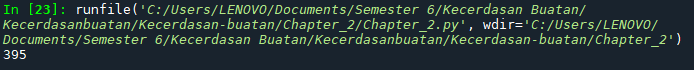
\includegraphics[width=11cm,height=2cm]{figures/Cp2-a.png}
	\caption{Load Dataset}
	\label{penanda}
\end{figure}

\item Generate Binary Label
\newline Selanjutnya pada bagian ini digunakan untuk mendeklarasikan pass/fail pada suatu data yang berdasarkan G1+G2+G3 dengan ketentuan nilai pass = 30 dan pada variable bandung dideklarasikan jika baris dengan G1+G2+G3 ditambahkan, dan hasilnya sama dengan 35 maka axis nya 1.
\begin{figure}[!htbp]
	\centering
	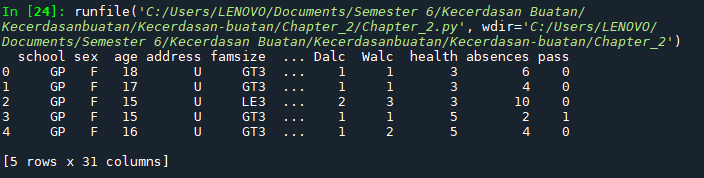
\includegraphics[width=13cm,height=5cm]{figures/Cp2-b.png}
	\caption{Generate Binary Label}
	\label{penanda}
\end{figure}

\item Use one-hot encoding on categorical columns 
\newline One-hot encoding merupakan proses dimana sebuah variable kategorikal dikonversikan menjadi bentuk yang dapat disediakan oleh algoritma Machine Learning untuk dapat melakukan pekerjaan yang lebih baik dalam memprediksi. Disini menggunakan fungsi panda pdgetdummies untuk jenis kelamin, sekolah, alamat dan lainnya. Metode head ini digunakan untuk mengembalikan baris n atas 5 secara default dari frame atau seri datanya.
\begin{figure}[!htbp]
	\centering
	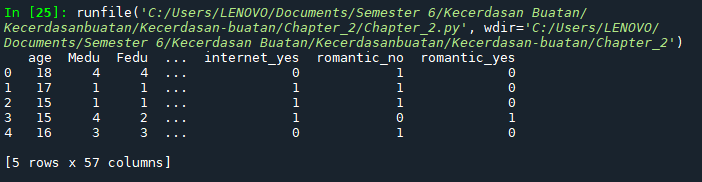
\includegraphics[width=12cm,height=4cm]{figures/Cp2-c.png}
	\caption{Use one-hot encoding on categorical columns}
	\label{penanda}
\end{figure}

\item Shuffle Rows
\newline Pada shuffle rows ini ditujukan untuk mengembalikkan sample secara tidak teratur dari objek. Terdapat train dan test yang digunakan untuk membagi train, test dan kemudian dibagi lagi train ke validasi dan test. kemudian di import sebuah modul numpy sebagai np yang digunakan untuk mengembalikan nilai passing dari pelajar dan dari keseluruhan dataset dengan menggunakan print.
\begin{figure}[!htbp]
	\centering
	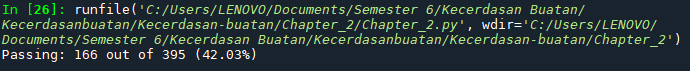
\includegraphics[width=14cm,height=2cm]{figures/Cp2-d.png}
	\caption{Shuffle Rows}
	\label{penanda}
\end{figure}

\item Fit a decision tree
\newline Import modul tree dari library scikit-learn. Dan selanjutnya nanti akan mendefinisikan variable menggunakan decision classifier. Di dalam variable itulah terdapat criterion yang merupakan suatu fungsi untuk mengukur kualitas split. Agar decision tree classifier dapat di jalankan maka gunakan perintah fit
\begin{figure}[!htbp]
	\centering
	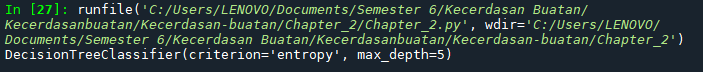
\includegraphics[width=14cm,height=2cm]{figures/Cp2-e.png}
	\caption{Fit a decision tree}
	\label{penanda}
\end{figure}

\item Visualize tree
\newline Konsep dari decision tree adalah mengubah data menjadi aturan-aturan keputusan. Manfaat utama dari penggunaan decision tree adalah kemampuannya untuk mem-break down proses pengambilan keputusan yang kompleks menjadi lebih simple, sehingga pengambil keputusan akan lebih menginterpretasikan solusi dari permasalahan. Graphviz yaitu suatu perangkat lunak visualisasi grafik objek open source. Visualisasi grafik merupakan cara untuk mewakili informasi struktural sebagai diagram grafik dan jaringan abstrak. treeexportgraphviz merupakan sebuah fungsi yang akan menghasilkan representasi Graphviz dari decision tree,kemudian ditulis kedalam out file, sehingga akan ditampilkan sebuah diagram grafik bercabang.
\begin{figure}[!htbp]
	\centering
	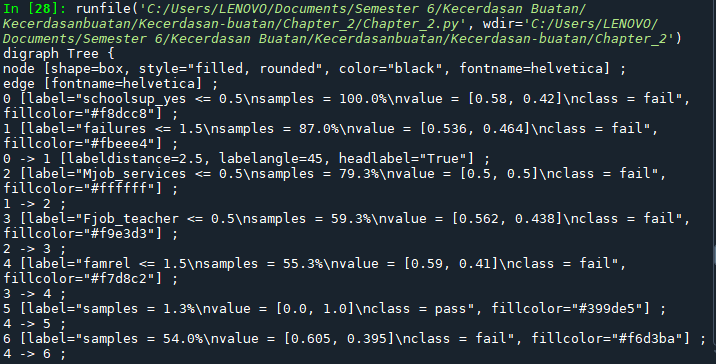
\includegraphics[width=17cm,height=4cm]{figures/Cp2-f.png}
	\caption{Visualize tree - graph}
	\label{penanda}
\end{figure}

\item Save Tree
\newline TREEEXPORTGRAPHVIZ merupakan sebuah fungsi yang akan menghasilkan representasi graphviz dari decision tree yang kemudian akan di tulis ke dalam sebuah outfile. Di dalam file tersebut akan disimpan classifier nya kemudian mengekspor file tersebut dengan namastudent performance kedalam folder tujuan kemudian jika salah maka akan mengembalikan nilai fail.


\item Score
\newline Score biasa di kenal sebagai prediksi atau proses yang nantinya dapat menghasilkan nilai berdasarkan pada model pembelajaran mesin yang terlatih dan diberi beberapa data input baru. Nilai dibuat untuk mewakili prediksi nilai di masa depan atau juga dapat mewakili kategori serta hasil yang mungkin. Dalam hal ini variable solo akan memprediksi nilai bandung test att dan test pass.
\begin{figure}[!htbp]
	\centering
	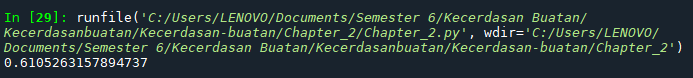
\includegraphics[width=14cm,height=2cm]{figures/Cp2-g.png}
	\caption{Score}
	\label{penanda}
\end{figure}


\item Evaluasi Score - Cross Val Score
\newline di dalam Evaluasi Score, di script ini akan mengevaluasi score dengan menggunakan validasi silang. 
\begin{figure}[!htbp]
	\centering
	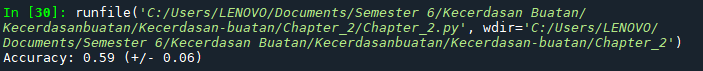
\includegraphics[width=14cm,height=2cm]{figures/Cp2-h.png}
	\caption{Evaluasi Score - Cross Val Score}
	\label{penanda}
\end{figure}

\item Max Depth
\newline Script berikut dapat menunjukkan bahwa semakin banyak tree maka semakin banyak perpecahan yang dimiliki dan akan lebih banyak menangkap informasi dari data. Variable solo disini akan mendefinisikan tree kemudian variable jakarta akan mengevaluasi score nya dengan validasi silang. Kemudian akan di definisikan decision tree dengan kedalaman mulai dari 1 hingga 20 dan
merencanakan pelatihan dan menguji skor auc.
\begin{figure}[!htbp]
	\centering
	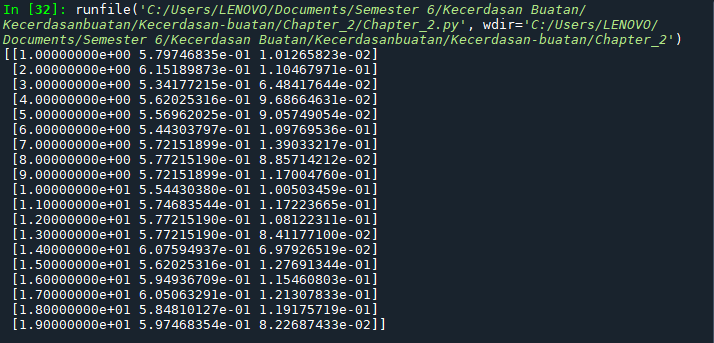
\includegraphics[width=10cm,height=7cm]{figures/Cp2-i.png}
	\caption{Max Depth}
	\label{penanda}
\end{figure}

\item Depth In Range
\newline Depth acc membuat array kosong dengan mengembalikan array baru menggunakan bentuk dan tipe yang diberikan, tanpa menginisialisasi entri. Dengan 19 sebagai bentuk array kosong, 3 sebagai output data-type dan float urutan kolom utama (gaya Fortran) dalam memori. Variabel solo yang akan melakukan
split score dan jakarta akan mengvalidasi score secara silang. Kemudian jakarta std yaitu menghitung standar deviasi dari data yang diberikan (elemen array) di sepanjang sumbu yang ditentukan (jika ada).
\begin{figure}[!htbp]
	\centering
	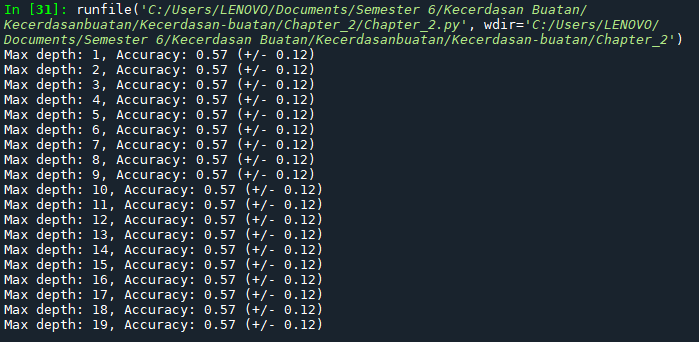
\includegraphics[width=10cm,height=8cm]{figures/Cp2-j.png}
	\caption{Depth In Range}
	\label{penanda}
\end{figure}

\item Matplotlib
\newline Contoh gambar ini akan di import sebuah library dari matplotlib yaitu pylot sebagai plt, fig dan ax yang menggunakan subplots untuk dapat membuat gambar serta satu set subplot. axerrorbar dalam script akan membuat error bar kemudian membuat sebuah grafik yang akan ditampilkan menggunakan perintah show.
\begin{figure}[!htbp]
	\centering
	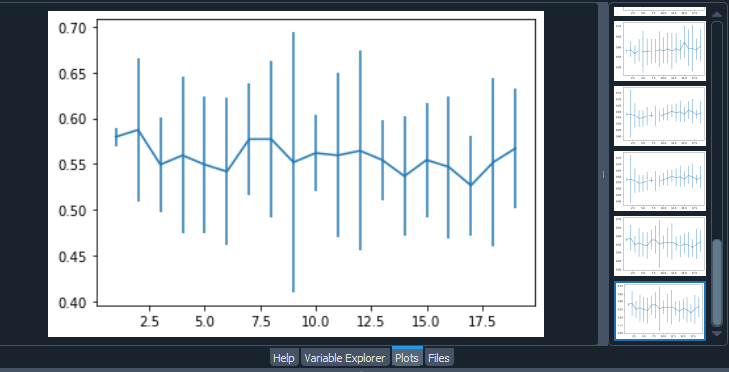
\includegraphics[width=10cm,height=6cm]{figures/Cp2-k.png}
	\caption{Matplotlib}
	\label{penanda}
\end{figure}
\end{enumerate}